\subsection{Experimental Evaluation}
\label{rasc:sec:eval}

We address the following research questions: 
\begin{enumerate}
    \item How efficient is \sysname's polling technique? (\Cref{rasc:sec:detection_times})
    \item Does action length estimation converge? (\Cref{rasc:sec:training-eval}) 
    \item If the action length distribution evolves, can \sysname{} reconverge its learnt distribution quickly? (\Cref{rasc:sec:training-eval})
    \item When actions are interrupted, can \sysname{} distinguish them from a scenario where they actually fail? (\Cref{rasc:sec:interruption-eval})
    \item Under realistic routines, how do \scheduler+\{RV, STF\} compare to baselines~\cite{SafeHomeEuroSys2021} {in latency \& overhead}? (\Cref{rasc:sec:sched-finetuning})
\end{enumerate}

\noindent {\bf Trace Collection.} 
To drive our trace-driven emulation, we collected traces of (I) device action times that form a diverse set of devices in an office building, and (II) a set of diverse routines, inspired by existing routine datasets including IoTBench~\cite{iotbench,smartthingsapps}, described in \Cref{rasc:sec:sched-finetuning}.
For (I), we manually collected a significant dataset of action completion times. We recorded multiple ($>50$) trials over 5 days, with 2 elevators, 2 projector screens, 2 lights, 2 doors, and 4 shades. Elevator data was collected while other users were using it, and thermostat traces are from an existing dataset~\cite{fraunhofer_thermostat_2022}.  

\subsubsection{\sysname{} Polling Efficiency}
\label{rasc:sec:detection_times}

We compare \sysname's adaptive polling efficiency to a baseline periodic polling strategy, which polls every $Q_w$.
\Cref{rasc:fig:polls-per-action} shows that compared to periodic polling, adaptive polling uses 44\% to 89\% fewer polls to detect the action completion. 
We set the Service Level Objective or $SLO$---the percentage of events \sysname{} promises to detect within $Q_w$ (\Cref{rasc:algo:adaptive-polling-algorithm})---%
to 0.9 and $Q_w$ equal to 2, 3, and 30 (seconds) for door, shade, and thermostat actions, respectively.
Action \texttt{shade down}'s detection time is higher with adaptive polling but still below $Q_w$. This data point highlights the following tradeoff: periodic polling is costly and guarantees detection within $Q_w$ always, whereas adaptive polling is very cost-efficient but may detect action progress within $Q_w$ only with high probability ($\ge SLO$).

\begin{figure}[tb!]
    \centering
    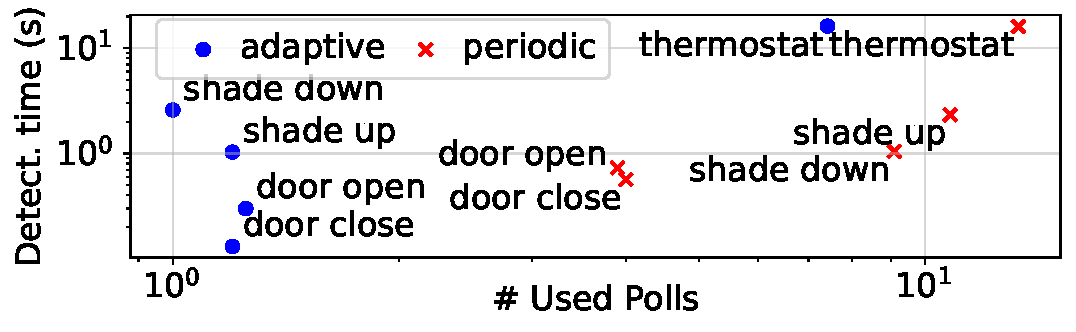
\includegraphics[width=0.7\linewidth]{RASC/figures/evaluation/rascal_poll_efficiency_scatter_plot.pdf}
    \caption{\bf \small \sysname's Adaptive Polling vs. Baseline Periodic Polling. \it \sysname{} is better (lower and to the left) in 4 of 5 cases. 
    }
    \medskip
    \label{rasc:fig:polls-per-action}
\end{figure}

\begin{table}[tb!]
    \centering
    \small
    % \setlength{\tabcolsep}{2pt}
    \renewcommand{\arraystretch}{1.02}
    % \tagpdfsetup{table/header-rows={1,2},table/header-columns={1}}
    \tagpdfsetup{table-tagging=false}
    \caption{\bf \small {\sysname's Adaptive Polling vs. Baseline V-opt-calculated Polling, Detection vs. Computation Time. All times are in seconds. Bold font indicates the lowest value for each action/metric combination. \it \sysname{} has similar detection times, but V-opt's computation time is impractical, especially for long actions.}}
    \bigskip
    \label{rasc:tab:V-opt}
    \begin{tabular}{|l||r|c|c|c|c|r|}
        \hline
        \multirow{2}{*}{\textbf{Action}} & \centering \textbf{Avg.} & \multicolumn{2}{c|}{\textbf{Detection Time}} & \multicolumn{2}{c|}{\textbf{Computation Time}} & \multirow{2}{*}{\textbf{Speedup}} \\
        \cline{3-6}  % Line only under columns 4 through 7
           & \textbf{Length} &      Adaptive &  V-opt         & Adaptive          & V-opt     & \\
        \hline\hline
        Door close  &   3.19 & 0.19          & \textbf{0.13} & \textbf{6.04e-04} & 4.38e-02 & 59.37 \\ \hline
        Door open   &   3.06 & \textbf{0.19} &  0.30         & \textbf{6.43e-04} & 3.82e-02 & 72.56 \\ \hline
        Shade up    &  29.64 & \textbf{0.31} &  1.02         & \textbf{3.96e-02} & 1.97e+01 & 497.77 \\ \hline
        Shade down  &  27.45 & \textbf{1.54} &  2.58         & \textbf{2.93e-02} & 1.63e+01 & 554.99 \\ \hline
        Therm 68,69 & 432.17 & \textbf{16.19}&    --         & \textbf{9.04}     & {2hr+}   & 796.34 \\ \hline
    \end{tabular}
\end{table}

\begin{figure}[tb!]
    \centering
    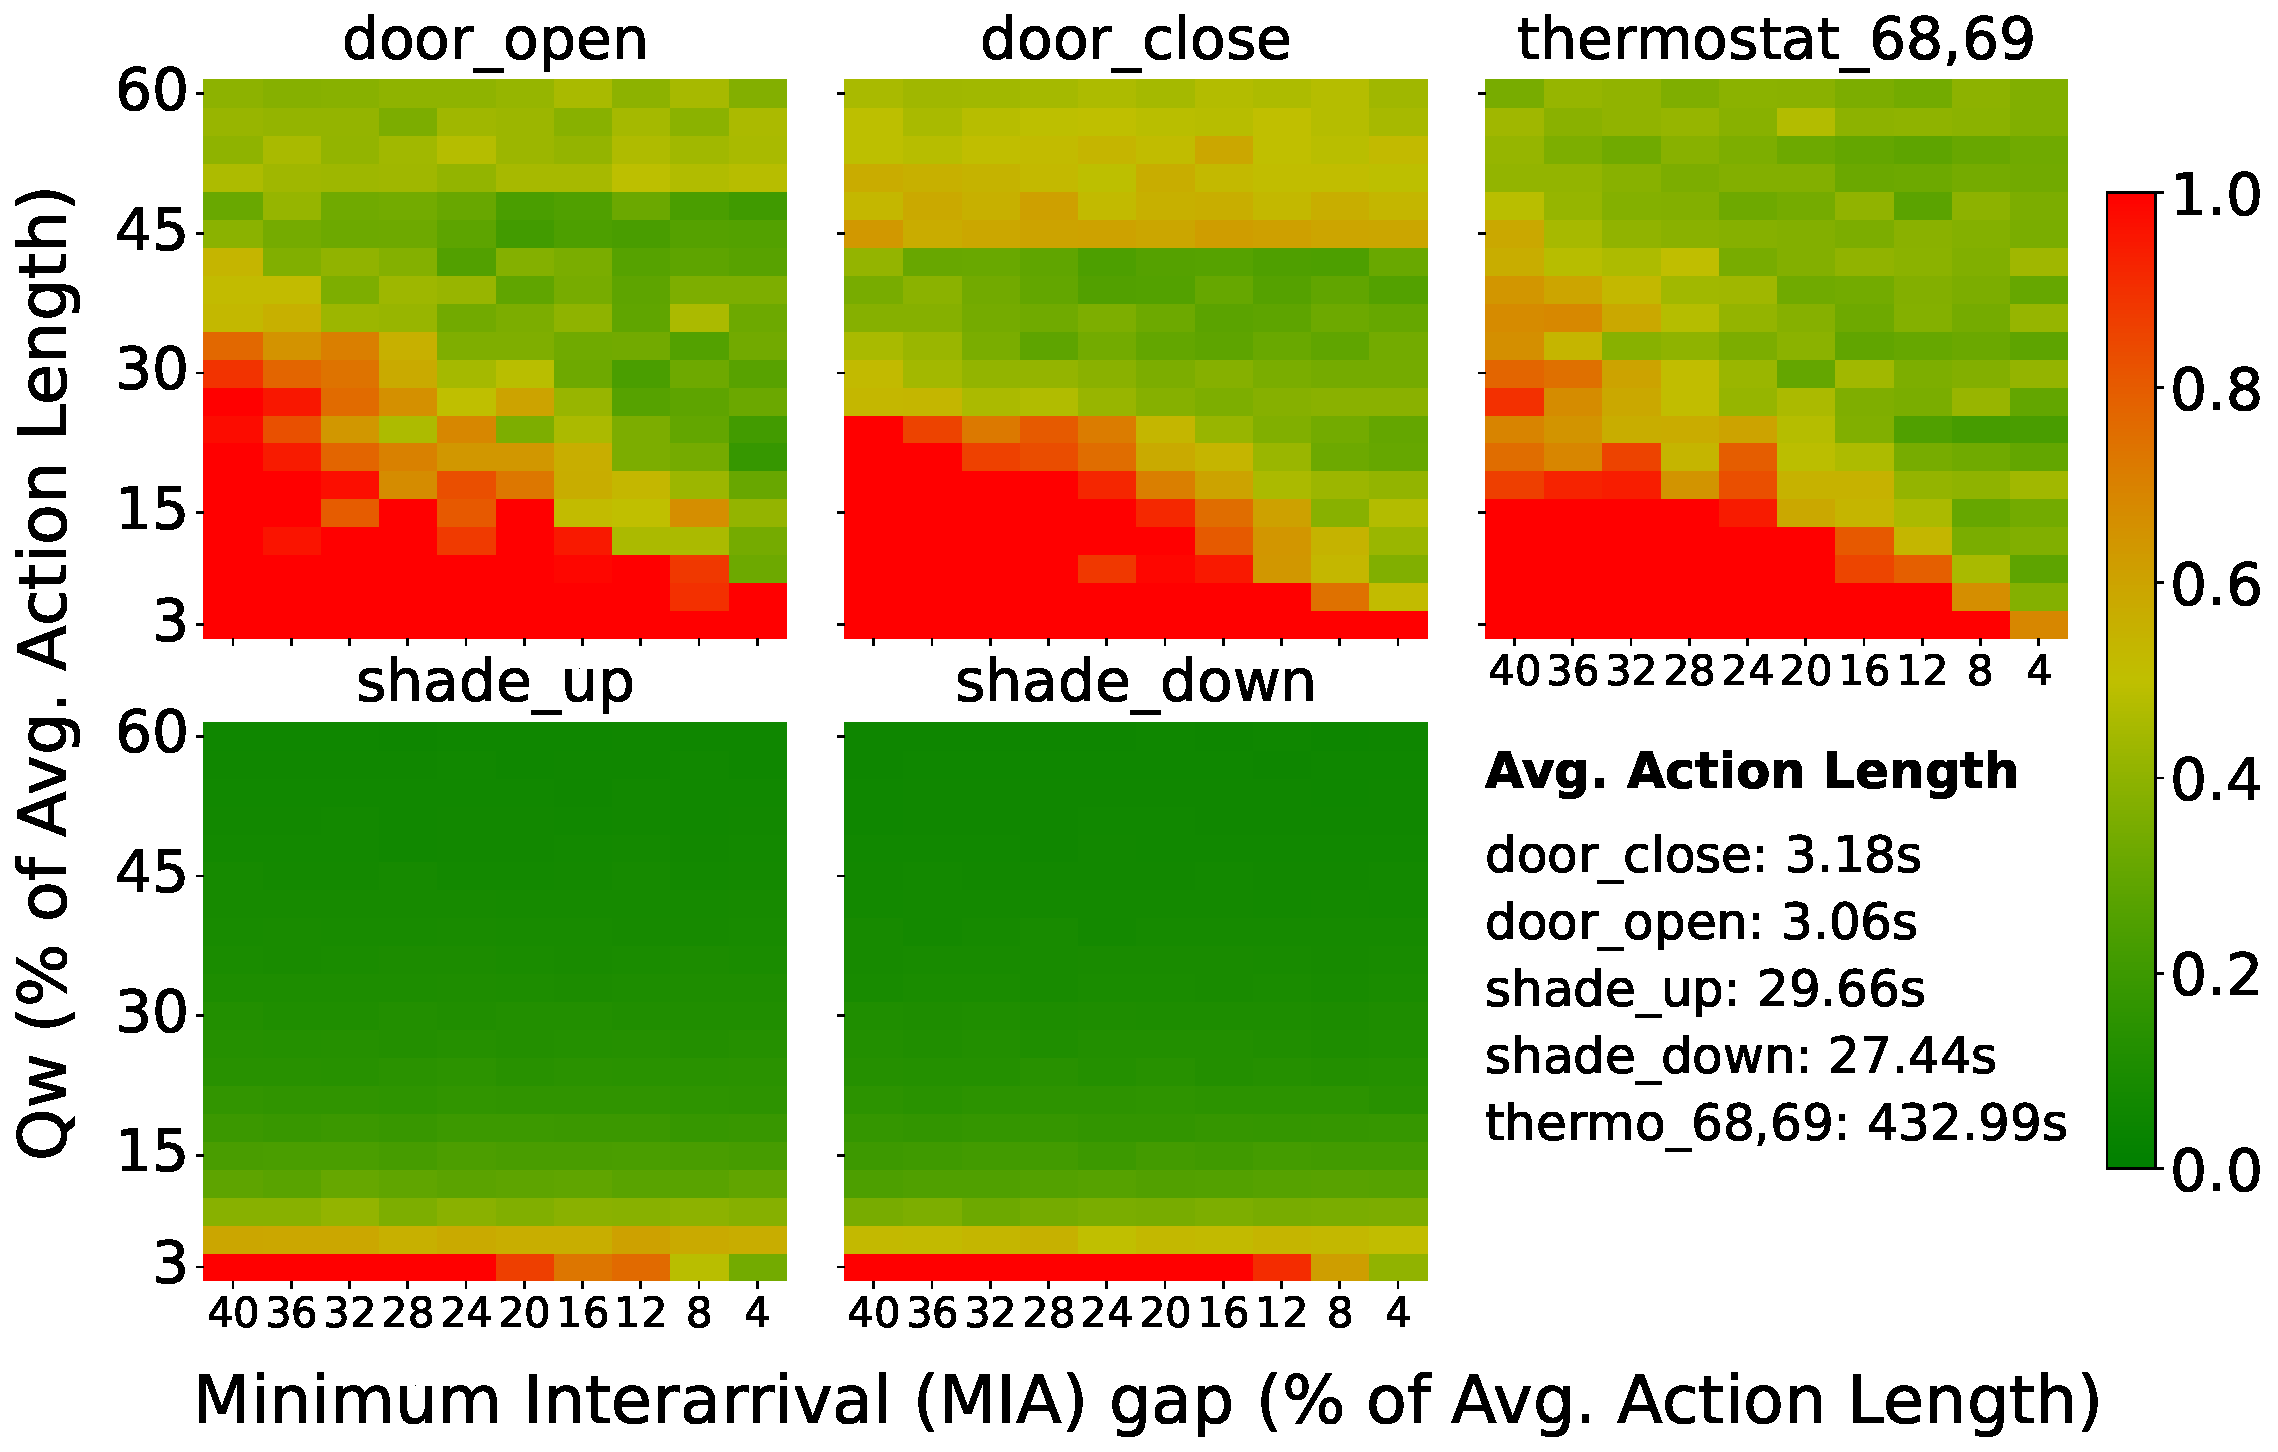
\includegraphics[width=0.7\linewidth]{RASC/figures/evaluation/MIA_results.pdf}
    \caption{\bf \small Effect of Extreme Rate Limiting: \sysname's Detection time under varying $Q_w$ (user-specified tolerance threshold).
    }
    \medskip
    \label{rasc:fig:rate-limiting}
\end{figure}

\Cref{rasc:tab:V-opt} compares \sysname's adaptive polling against the baseline called V-optimal (V-opt)~\cite{ioannidis1995balancing}, 
the classic dynamic-programming algorithm for histogram construction. V-opt selects bucket boundaries to minimize variance across bins. 
Both achieve comparable detection times, but \sysname{} computes poll placements 60-800$\times$ faster than V-opt.  
This efficiency gap makes V-opt impractical in real deployments; its computation time can exceed even the average action length (e.g., thermostat), while \sysname{} completes in milliseconds.

\Cref{rasc:fig:rate-limiting} shows the impact of device or API rate limits on \sysname's polling.
The x axis shows the API/device-imposed minimum inter-arrival (MIA) gap between consecutive polls. The y axis shows the user-specified tolerance threshold ($Q_w$). Both axes are normalized to average
action length.
The color is $min(\frac{detection\ time}{Q_w}, 1)$. Thus green and yellow indicate  detection time threshold being met. We observe that (i) for a given MIA, too stringent $Q_w$ values may not be satisfiable (red in plot); (ii) this $Q_w$ value threshold (for meeting 100\% detection: green in plot) drops quickly as MIA becomes less stringent (left to right);  and (iii) detection time for  uninterruptible mechanical actions 
(e.g., shade up \& down) is more tolerant to rate limiting, because uninterruptible actions have tighter (and thus predictable) action length distributions. 

\subsubsection{\sysname{} Training}
\label{rasc:sec:training-eval}

\noindent \textbf{Convergence Speed.} 
We measure how many action-length samples \sysname{} needs to reach a {\it stable} per-(device, action) distribution, 
%.We define ``stable'' as: 
i.e., mean and variance both differ by less than 5\% upon consecutive samples.
\Cref{rasc:fig:convergence} shows that 10-20 samples suffice across devices: actions lasting tens of seconds (door, elevator, shade, projector screen) converge in $\sim10$ samples, while longer actions (e.g., the 400\,s thermostat) require $\sim20$.

\begin{figure}[tb!]
    \centering
    \begin{subfigure}{0.49\linewidth}
        \centering
        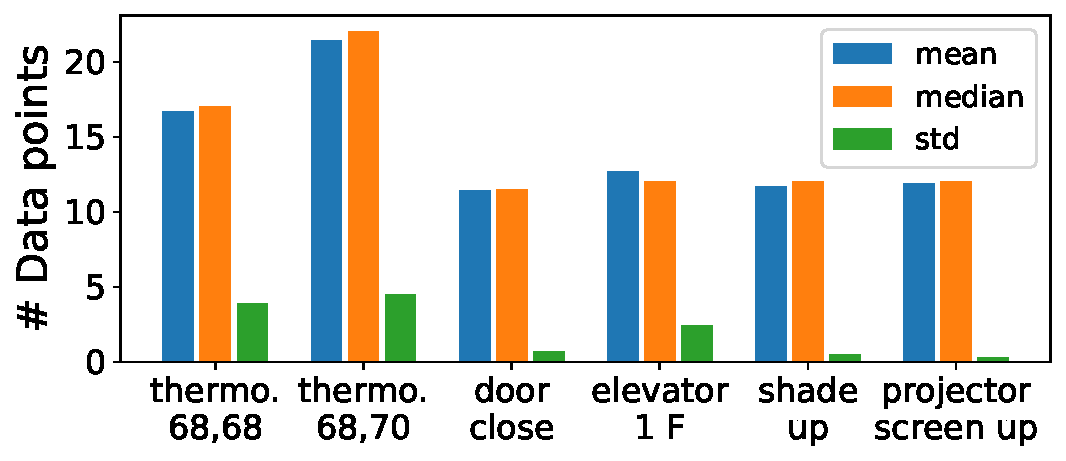
\includegraphics[width=\linewidth]{RASC/figures/evaluation/4_2_1.pdf}
        \caption{\small \sysname{} convergence time.}
        \label{rasc:fig:convergence}
    \end{subfigure}%
    \hfill
    \begin{subfigure}{0.49\linewidth}
        \centering
        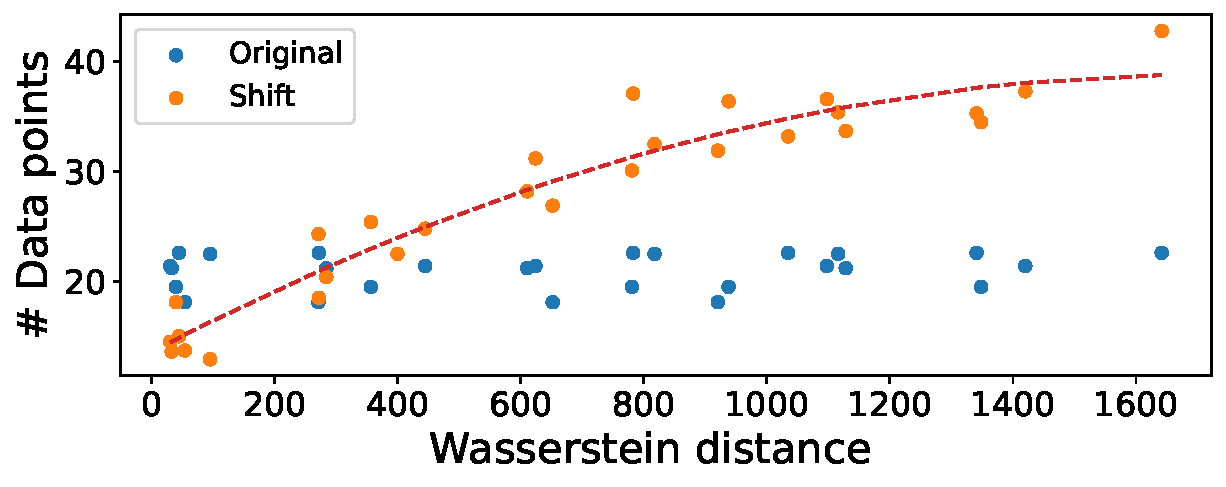
\includegraphics[width=\linewidth]{RASC/figures/evaluation/4_2_3.pdf}
        \caption{\small \sysname{} convergence  when action length drifts.}
        \label{rasc:fig:distribution-shift}
    \end{subfigure}
    \caption{\bf \small \sysname{} Convergence. \it \sysname{} converges quickly, requiring just over 20 (new) data points. }
    \medskip
    \label{rasc:fig:rasc-convergence}
\end{figure}

\begin{figure}[tb!]
    \centering
    \begin{subfigure}{0.49\linewidth}
        \centering
        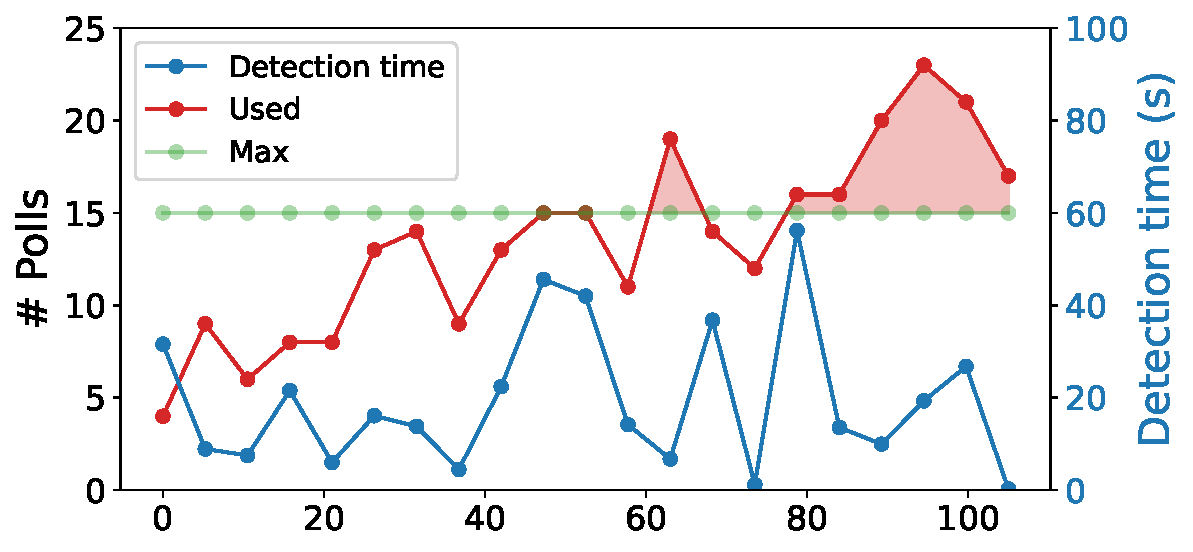
\includegraphics[width=\linewidth]{RASC/figures/evaluation/4_4_50_fixed.pdf}
        \caption{\small The interruption happens at the 50\% of the action.}
        \label{rasc:fig:action-interruption-fixed}
    \end{subfigure}%
    \hfill
    \begin{subfigure}{0.49\linewidth}
        \centering
        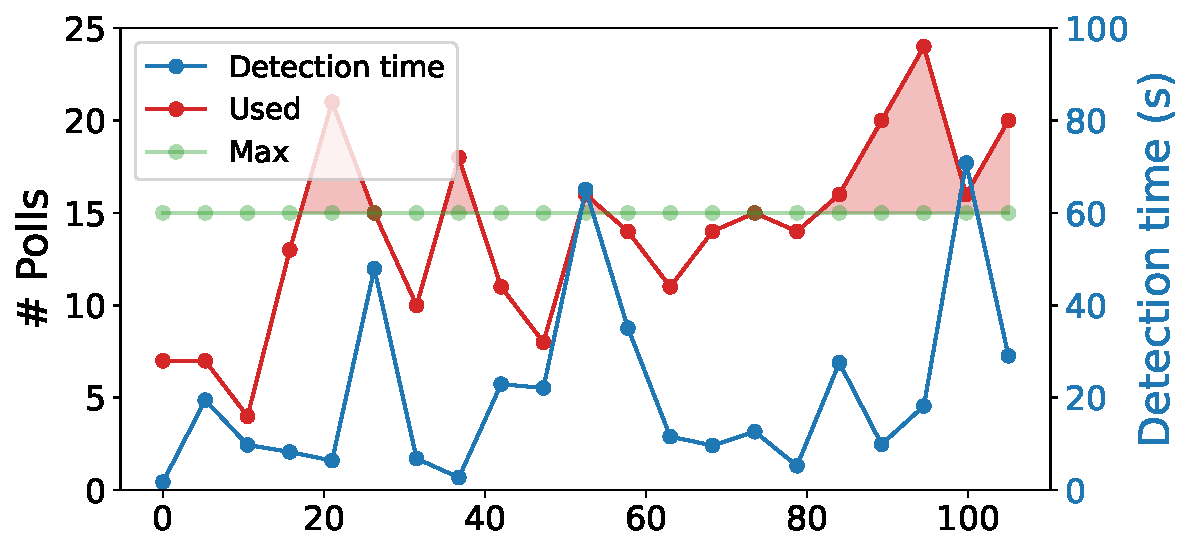
\includegraphics[width=\linewidth]{RASC/figures/evaluation/4_4_80_fixed.pdf}
        \caption{\small The interruption happens at the 80\% of the action.}
        \label{rasc:fig:action-interruption-fixed-80}
    \end{subfigure}
    \caption{\bf \small \sysname{} performance (polls) vs. Interruption Length relative to action length (\%).
    Action: thermostat from 68 to 69. {\it \sysname{} generally uses fewer polls than max. Exceptions: when interruptions are long (right side of plots).}}
    \label{rasc:fig:action-interruption}
\end{figure}

\begin{figure}[t!]
    \centering
    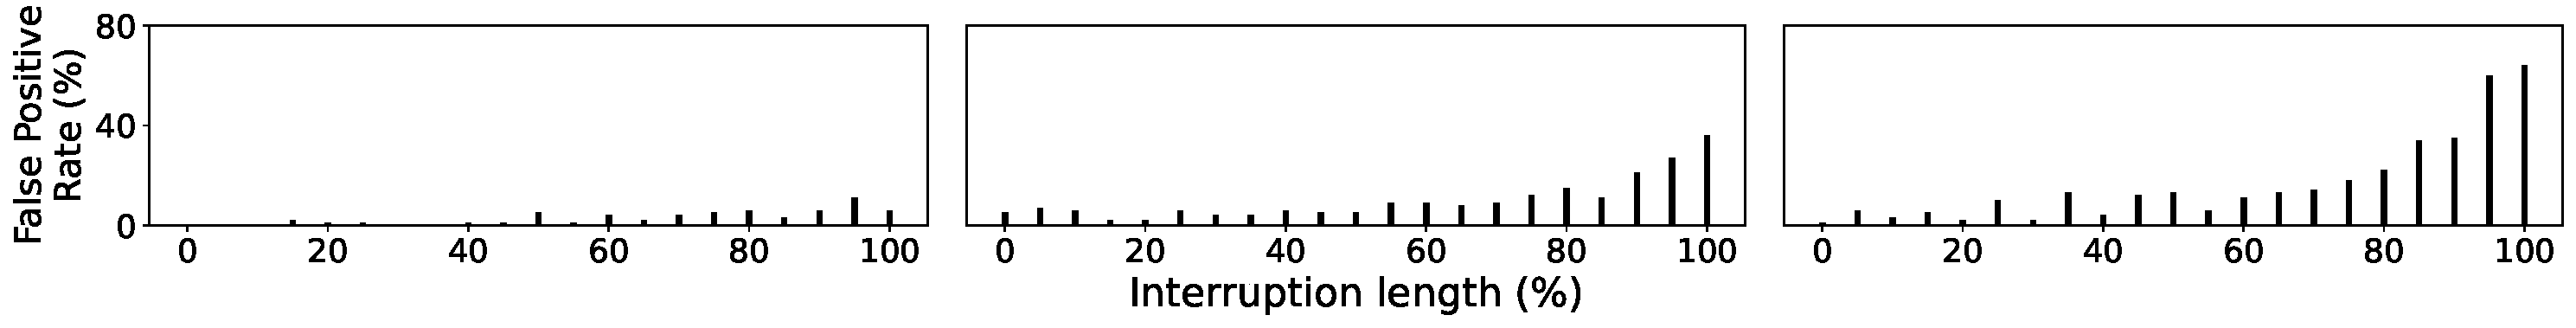
\includegraphics[width=\linewidth]{RASC/figures/evaluation/interruption.pdf}
    \caption{\bf \small Action Failure False Positive Rate during interruption. Left to right: interruption happens (resp.) at the 50\%, 80\%, and 90\% points of action. {\it False positives are generally low. Exception: when interruptions are long and towards the action's end. }}
    \medskip
    \label{rasc:fig:action-interruption-simulated}
\end{figure}


\noindent \textbf{Data Drift.} 
As devices get older, a single action's probability distributions for its progress points may start moving towards different ranges and probabilities.
How quickly can \sysname{}'s measurements catch up?  \Cref{rasc:fig:distribution-shift} measures (for a thermostat device, at various temperature settings) the Wasserstein (earthmover) distance~\cite{vaserstein1969,kantorovich1942}. This metric measures the distance between the real and learned distributions, for both the original distribution and the shifted distribution. We observe quick convergence, especially when the original distribution is $< 500$ (already a large value, much higher than the error in our measurements). 
For instance, the Wasserstein distance between the distributions from the door and the elevator is approximately 13.93. 
In reality, it is highly unlikely that a door would experience such significant degradation.

\subsubsection{Detecting Interrupted Actions}
\label{rasc:sec:interruption-eval}

Interruptions to ongoing actions are common due to environmental factors and human interactions.
\Cref{rasc:fig:action-interruption} shows a real deployment where a thermostat change (68$\rightarrow$69) is interrupted at 50\% and 80\% progress. 
The red area denotes extra polls beyond $U$. 
For early or brief interruptions, \sysname's overhead is low; with prolonged interruptions (right side of both plots), overhead rises, but detection time (blue line) stays low.

\Cref{rasc:fig:action-interruption-simulated} shows a simulation where we focus on {\it False Positive rate}, i.e., the percentage of experiments where \sysname{} {\it falsely} detected an action failure. 
We observe the False Positive rate rises with longer interruptions, especially when they occur near the action's end, indicating \sysname{} reliably distinguishes true failures from interruptions in most cases.

\subsubsection{Routine Scheduling}
\label{rasc:sec:sched-finetuning}

\begin{figure}[t!]
    \begin{subfigure}{0.49\linewidth}
        \centering
        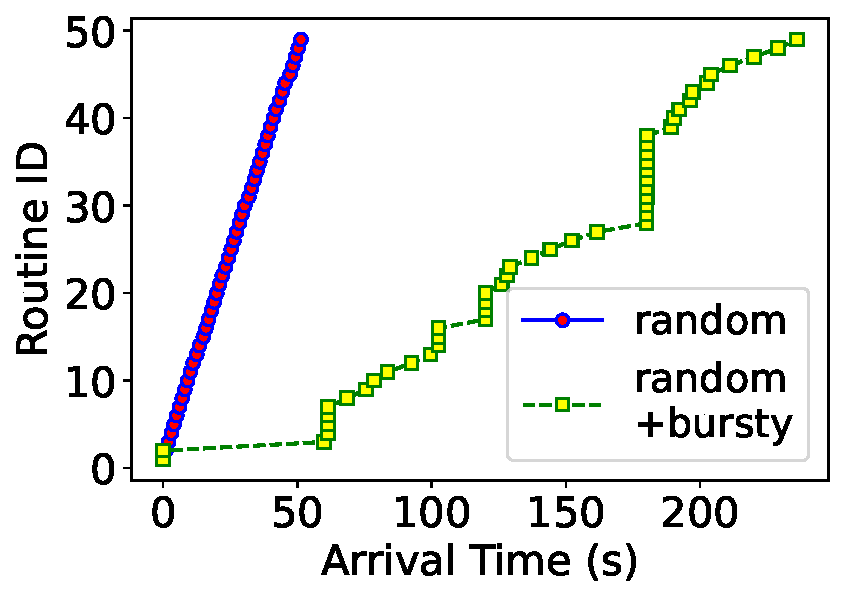
\includegraphics[width=0.8\linewidth]{RASC/figures/evaluation/arrival_times_plot.pdf}
        \captionsetup{width=.9\linewidth}
        \caption{\small The timeline of routine arrivals for the two datasets.}
        \label{rasc:fig:routine-arrival}
    \end{subfigure}%
    \hfill
    \begin{subfigure}{0.49\linewidth}
        \centering
        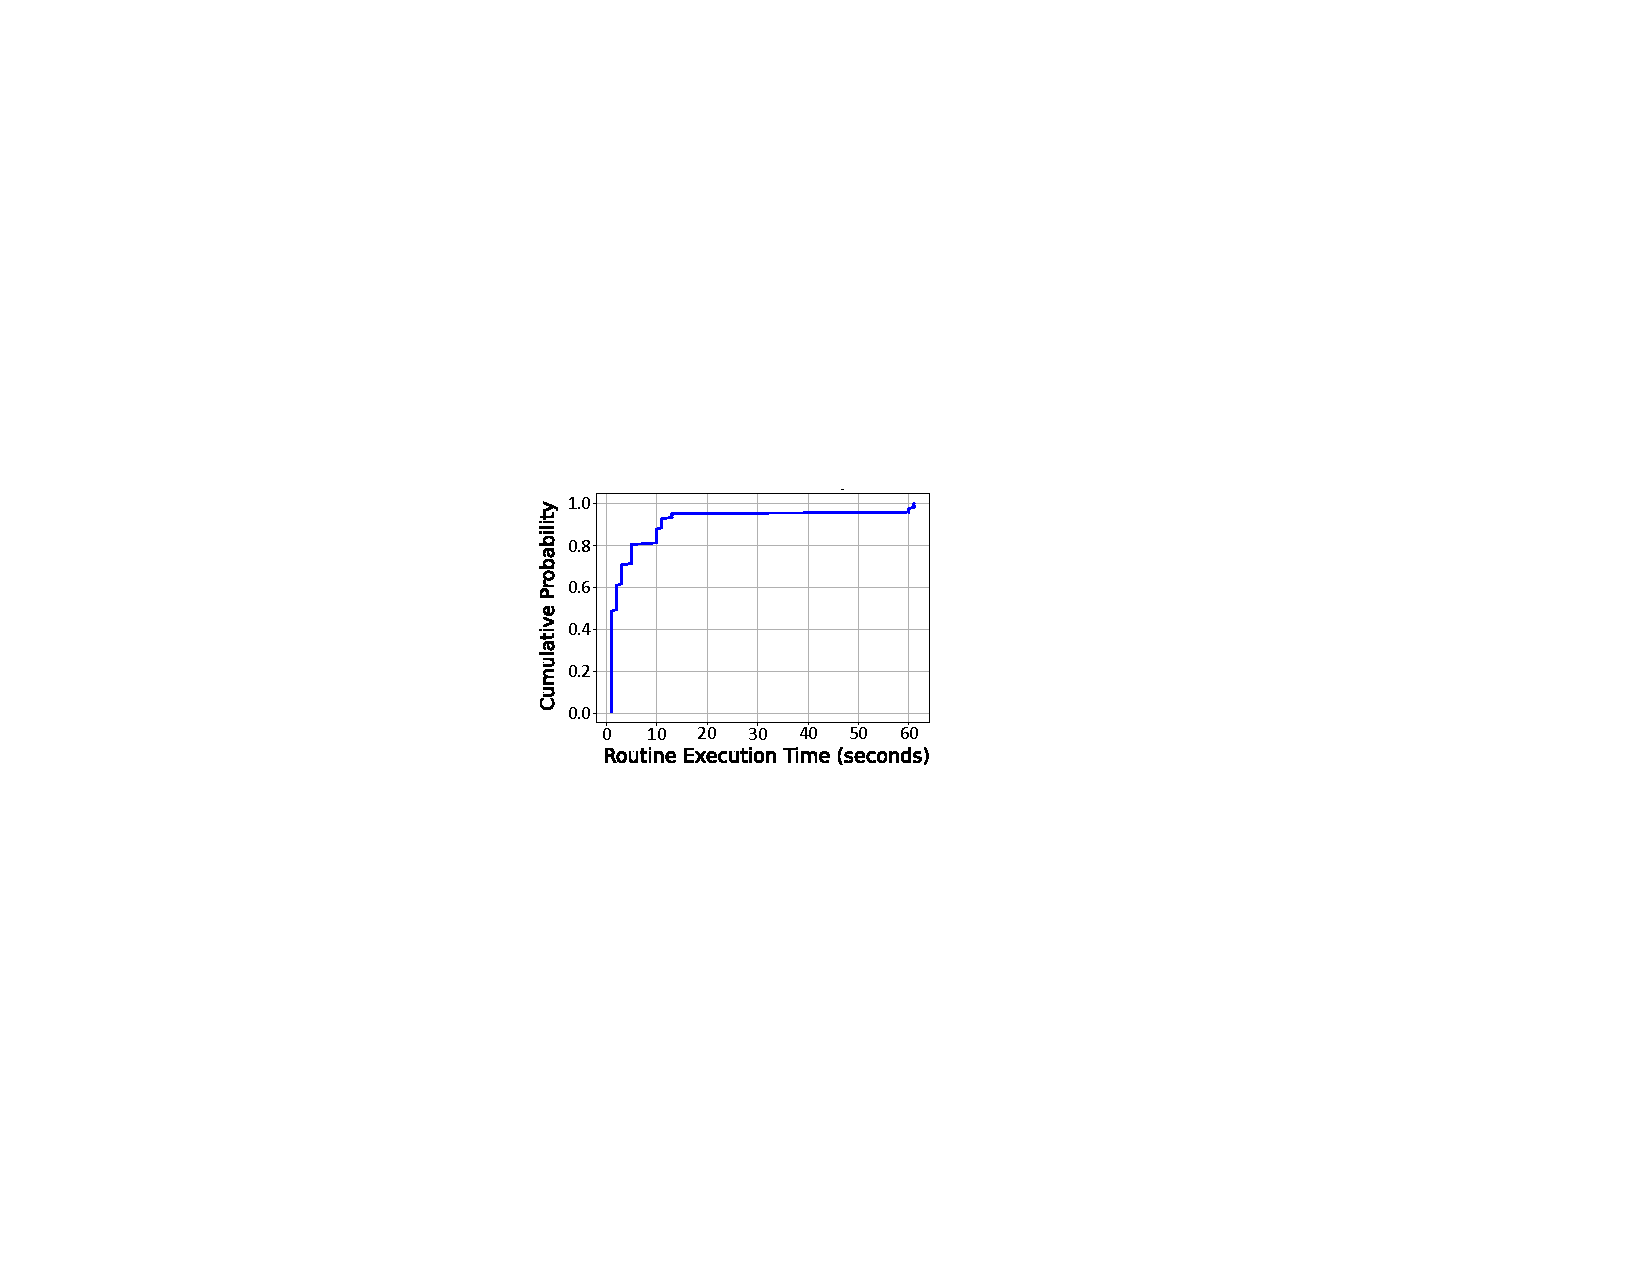
\includegraphics[width=0.8\linewidth]{RASC/figures/evaluation/cdf_action_len_larger_font.pdf}
        \caption{\small The sum of action lengths per routine as a CDF plot. }
        \label{rasc:fig:routine-action-lengths}
    \end{subfigure}
    \caption{\bf \small Our Routine Benchmark.
    }
    \medskip
    \label{rasc:fig:routine-dataset}
\end{figure}

We evaluate \sysname's end-to-end performance: overheads and comparing \scheduler{} scheduling (\Cref{rasc:sec:dyn-sched}) to baselines.

\noindent {\bf Dataset of Routines.}
We generated a suite of routines spanning diverse devices and lengths---statistics of our routine dataset are shown in \Cref{rasc:fig:routine-dataset}.
We have two arrival workloads: (1) {\it random}, attempting to capture ``background'' routine arrival throughout the 24 hours of a day, 
and (2)  {\it random+bursty}, a mix of 50\% random and 50\% bursty arrivals, 
intended to capture ``peak'' times of activity, such as morning, lunch, evening. 

\begin{table}[tb!]
    \centering
    \small
    % \setlength{\tabcolsep}{5pt}
    % \tagpdfsetup{table/header-rows={1,2},table/header-columns={1,2}}
    \tagpdfsetup{table-tagging=false}
    \caption{\bf \small \sysname's resource utilization under different polling strategies. Bold font indicates the lowest value for each dataset/ metric combination. {\it \sysname{} either incurs the lowest CPU or memory (among baselines), or is comparable to
    the lowest option.}}
    \bigskip
    \label{rasc:tab:resource-overheads}
    \begin{tabular}{|c|c|c|c|c|c|c|c|}
        \hline
        \multirow{2}{*}{Dataset} & \multirow{2}{*}{Polling Strategy} & \multicolumn{3}{c|}{CPU (\%)} & \multicolumn{3}{c|}{Memory (MB)} \\
        \cline{3-8}  % Line only under columns 3 through 8
         & & avg & q50 & q99 & avg & q50 & q99 \\
        \hline\hline
        \multirow{3}{*}{random} & adaptive & 8.79 & 1.8 & 19.8 & 4.12 & 4.73 & 8.33 \\
         & periodic & 9.6 & 8.6 & 24.06 & \textbf{3.36} & \textbf{3.33} & \textbf{6.22} \\
         & none & \textbf{2.41} & \textbf{1.1} & \textbf{10.1} & 17.72 & 19.19 & 20.28 \\
        \hline
        \multirow{3}{*}{random + bursty} & adaptive & 3.55 & 1.75 & \textbf{9.68} & \textbf{4.1} & \textbf{4.36} & \textbf{5.9} \\
         & periodic & 4.6 & 2.9 & 19.26 & 4.54 & 4.61 & 6.58 \\
         & none & \textbf{2.72} & \textbf{1.3} & 22.39 & 17.87 & 18.21 & 19.07 \\
        \hline
    \end{tabular}
\end{table}

\begin{figure}[tb!]
    \centering
    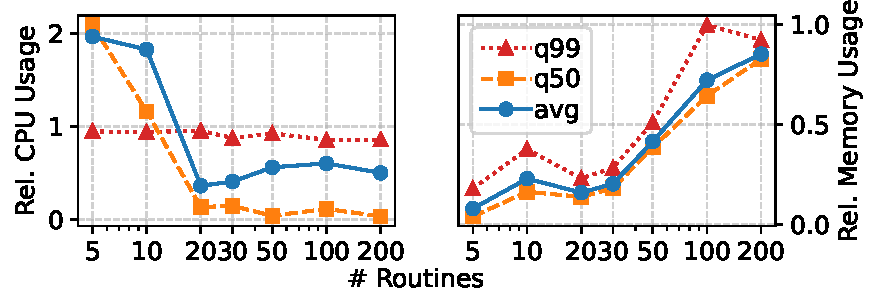
\includegraphics[width=0.7\linewidth]{RASC/figures/evaluation/rascal_scalability_overhead_norm_scale.pdf}
    \caption{\bf \small \sysname's relative resource utilization across varying routine loads. 
    {\it \sysname's CPU overhead is consistently low, while memory usage scales sub-linearly with the \# concurrent routines.}
    }
    \medskip
    \label{rasc:fig:scalability-overhead}
\end{figure}


\noindent \textbf{Overheads.} 
\Cref{rasc:tab:resource-overheads} reports \sysname{}'s process overhead under different polling strategies. 
Adaptive polling is consistently more efficient than periodic---up to 63\% lower CPU and 43\% lower memory. 
Disabling polling (\emph{none}) yields only marginal or inconsistent gains (CPU q99 up to 68\%, otherwise up to 33\%), and memory can be worse. In fact, memory is higher with no polling than with \sysname{}, indicating our automation-tracking memory management outperforms Home Assistant's baseline, which overuses external libraries.

\Cref{rasc:fig:scalability-overhead} illustrates \sysname's {\it relative} resource utilization, calculated as the ratio of utilization with \textit{adaptive} polling to utilization with polling disabled
(\textit{none}).
We vary concurrent routine load from smart home scale (up to 10) to smart buildings and campuses (up to 200).
Both \sysname's 99th percentile CPU \& all memory metrics %(\new{all metrics}) 
stay below that of disabled polling. While mean (median) %relative 
CPU usage  peaks at $\sim2\times$  at low loads (up to 20 routines) due to fixed scheduling 
upfront \sysname{} overhead, 
% beyond 20 %concurrent 
% routines 
it then drops, stabilizing at $\sim0.6\times$ ($\sim0.1\times$).
Relative memory rises with load but plateaus with 200 % concurrent 
routines at $\sim0.8\times$. This is the resource vs. benefit tradeoff entailed by \sysname.
%Thus \sysname{} is CPU- and memory-efficient.%

\begin{figure}[t]
  \centering

  \begin{minipage}[b]{0.55\textwidth}
    \centering
    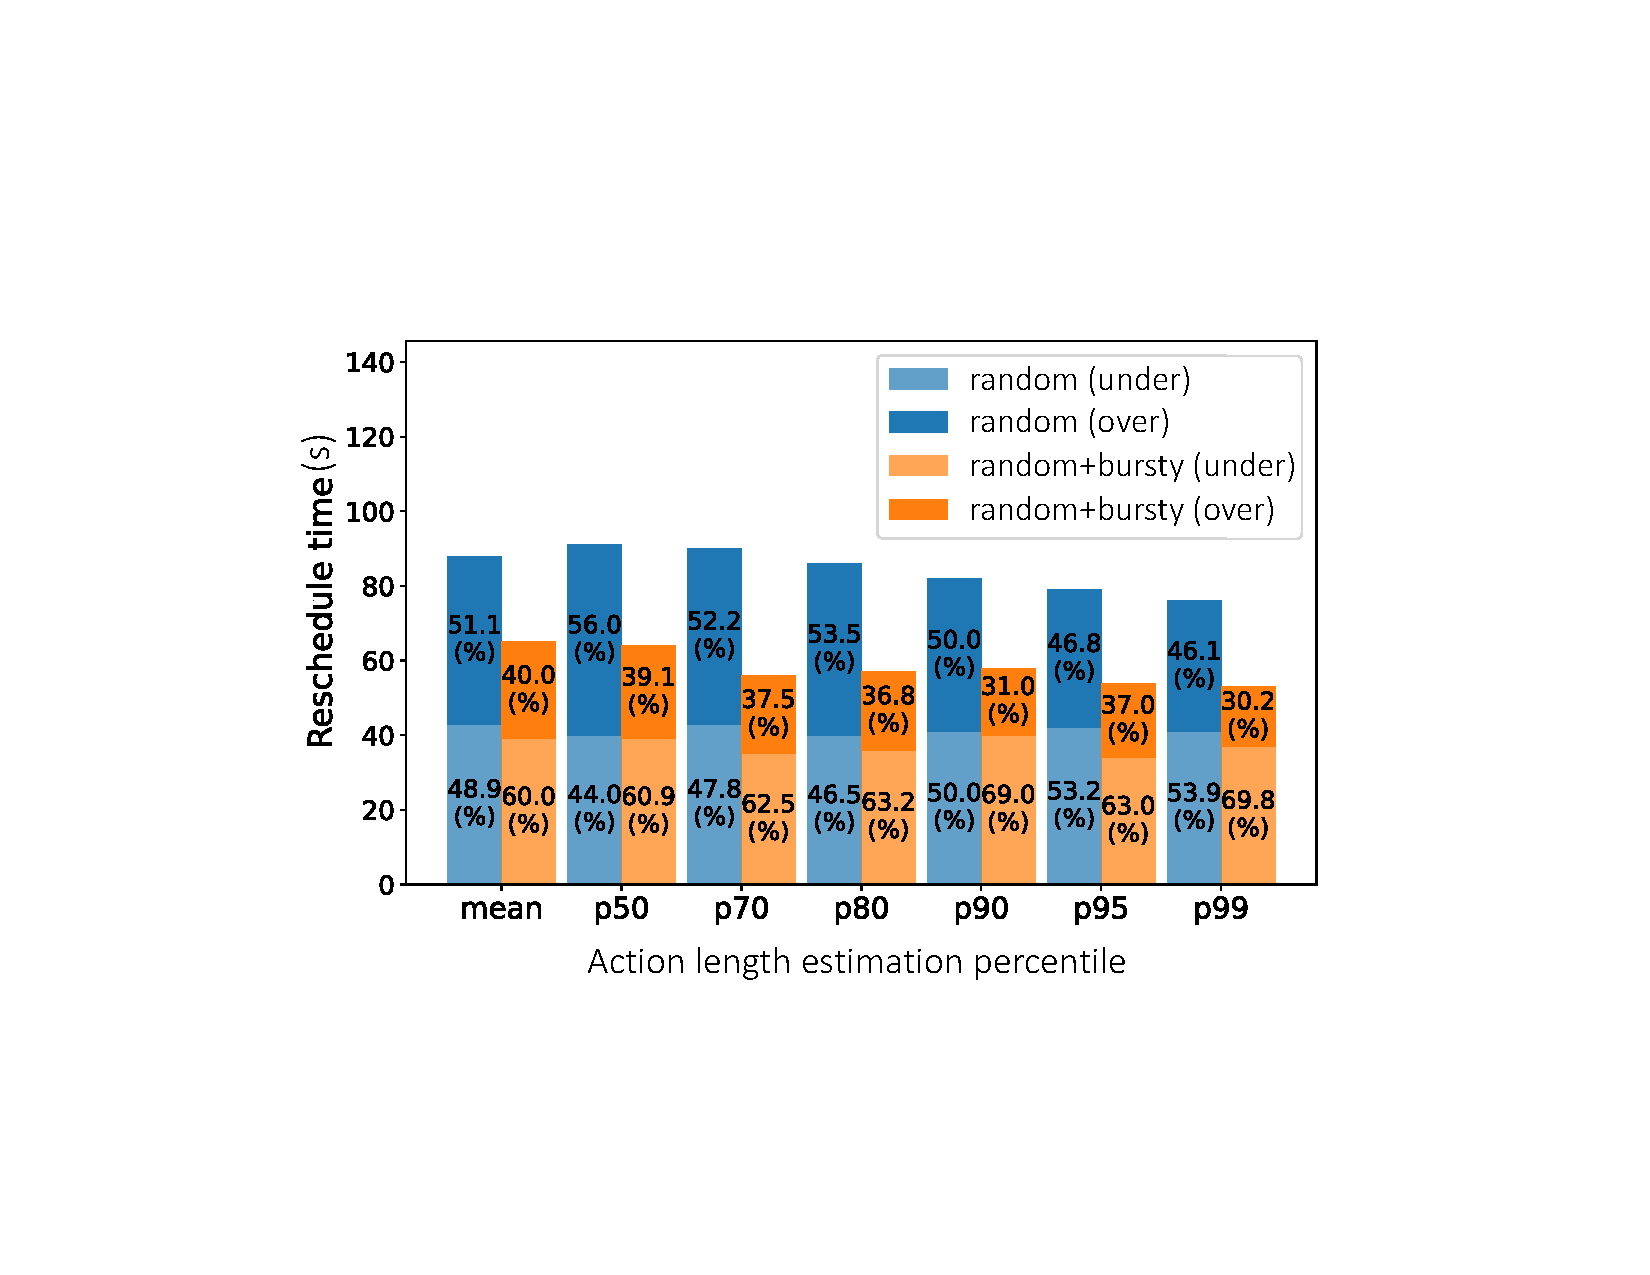
\includegraphics[width=\linewidth]{RASC/figures/evaluation/7_5_x-axis_new-ds.pdf}
    \captionof{figure}{\bf \small Rescheduling Overhead.
    Bars show total rescheduling time over the dataset, split into under-/over-time handling. {\it \sysname{} overhead stays low.}}
    \label{rasc:fig:reschedule_overhead}
  \end{minipage}
  \hfill
  \begin{minipage}[b]{0.39\textwidth}
    \centering
    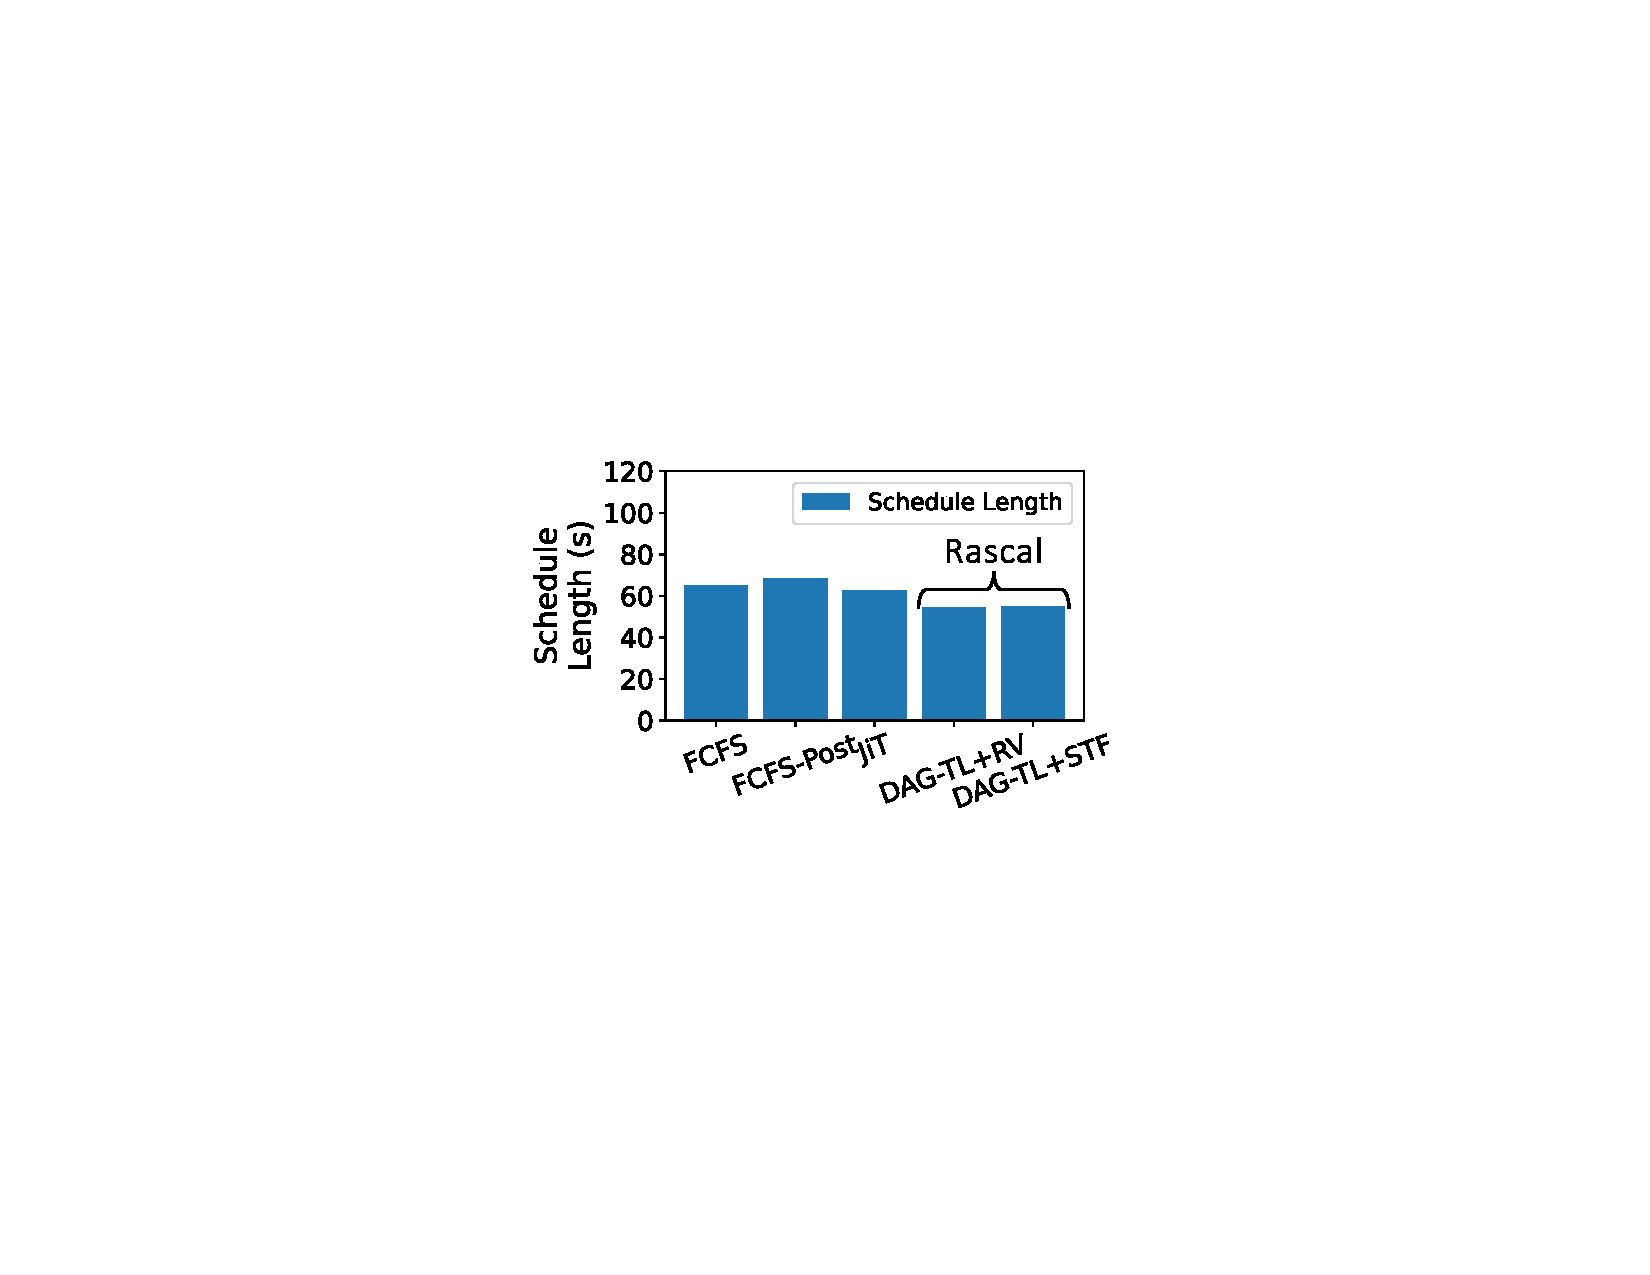
\includegraphics[width=\linewidth]{RASC/figures/evaluation/schedule_metric_Schedule Length_rascal.pdf}
    \captionof{figure}{\small \bf Schedule length comparison.
    {\it \sysname{} (right two) creates at least 11\% faster schedules vs. Baselines (left three).}
    }
    \label{rasc:fig:sched_len_comparison}
  \end{minipage}
\end{figure}

\Cref{rasc:fig:reschedule_overhead} shows \sysname's rescheduling overheads with STF (Shortest Task First). For both datasets, rescheduling time drops 
as action-length estimates increase, indicating that overestimation reduces overhead---even with more early completions. 
The random+bursty dataset achieves faster rescheduling time as the schedule is tighter at times and traversals are faster. 

\label{rasc:sec:sched-comparisons}



\begin{figure}[t]
    \begin{minipage}[t]{0.49\textwidth}
        \centering
        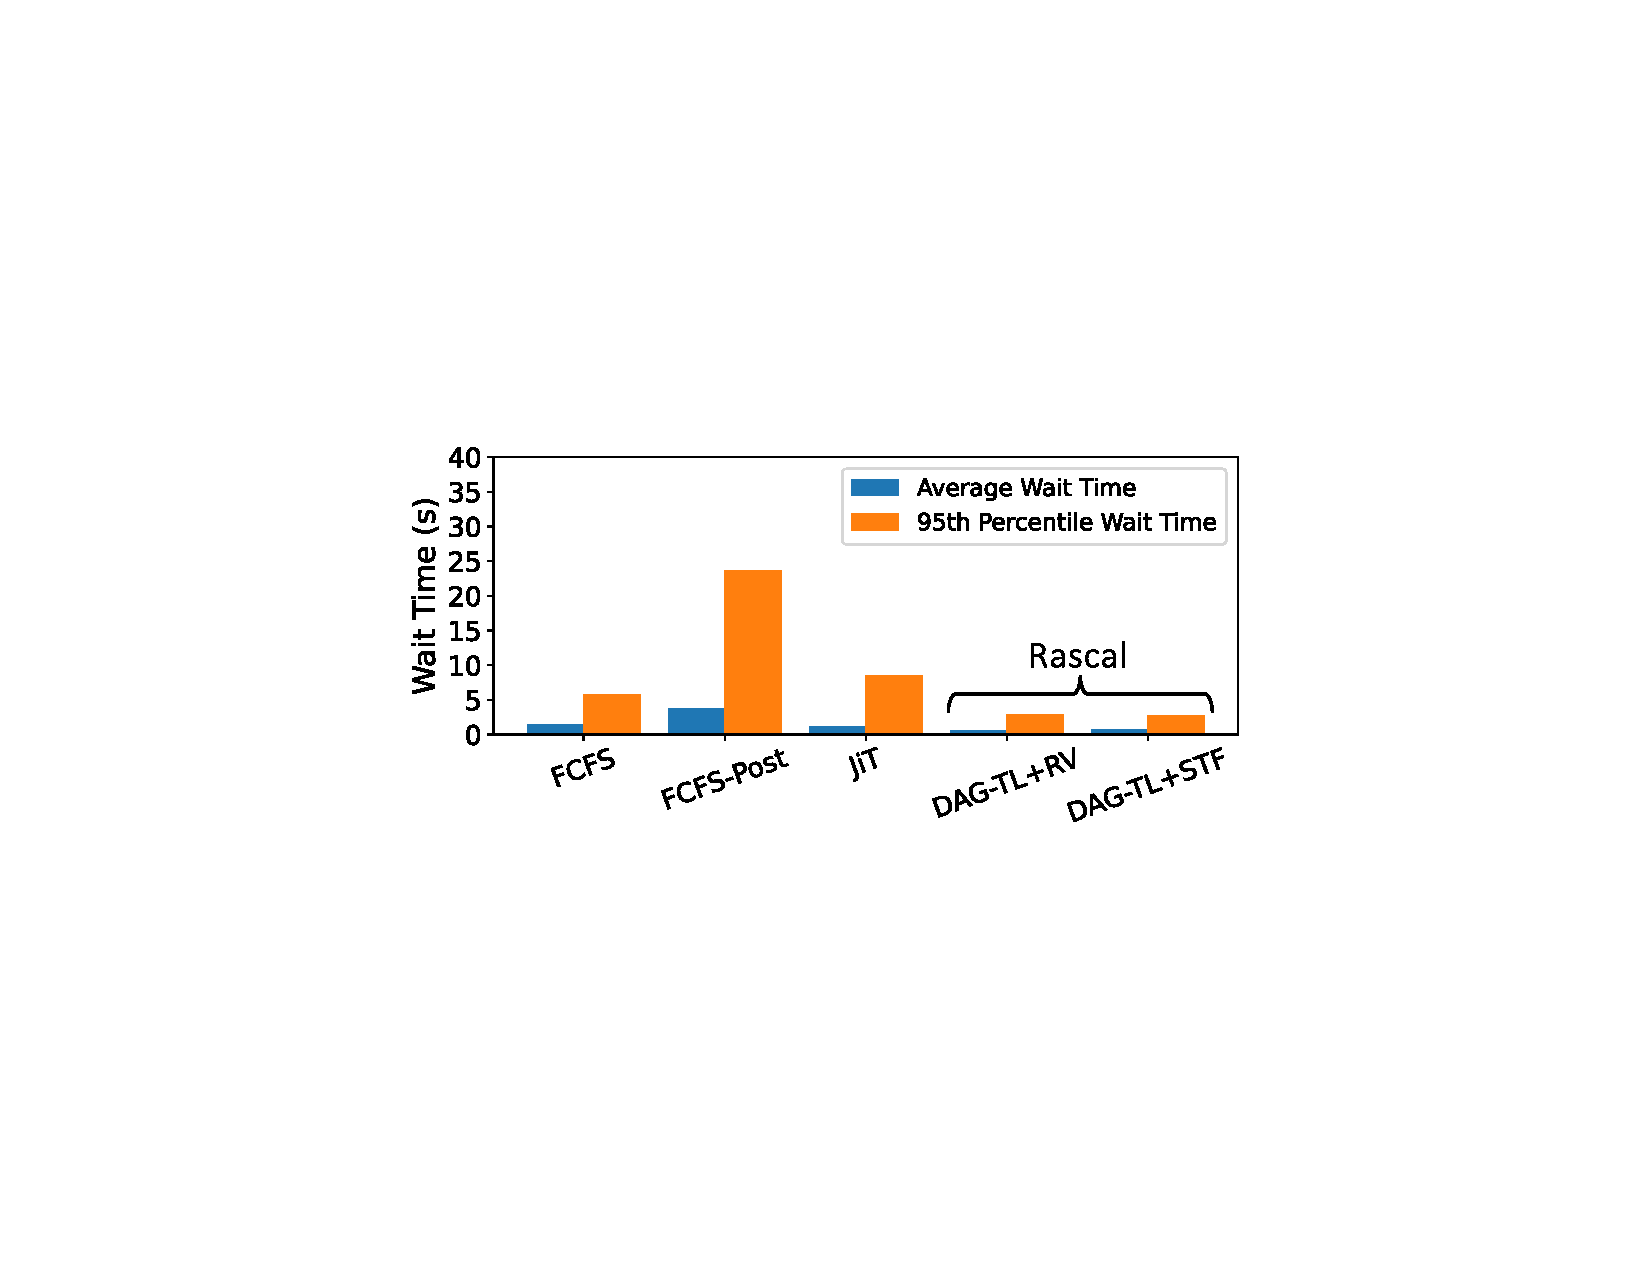
\includegraphics[width=\linewidth]{RASC/figures/evaluation/schedule_metric_Wait Time_rascal.pdf}
        \captionof{figure}{\small \bf 
        Wait time comparison. {\it \sysname{} (right two groups) decreases wait times by at least 33\% and 50\% for mean and q95 values, respectively, vs. Baselines (three left groups).}
        }
        \label{rasc:fig:wait_time_comparison}
    \end{minipage}
    \hfill
    \begin{minipage}[t]{0.49\textwidth}
        \centering
        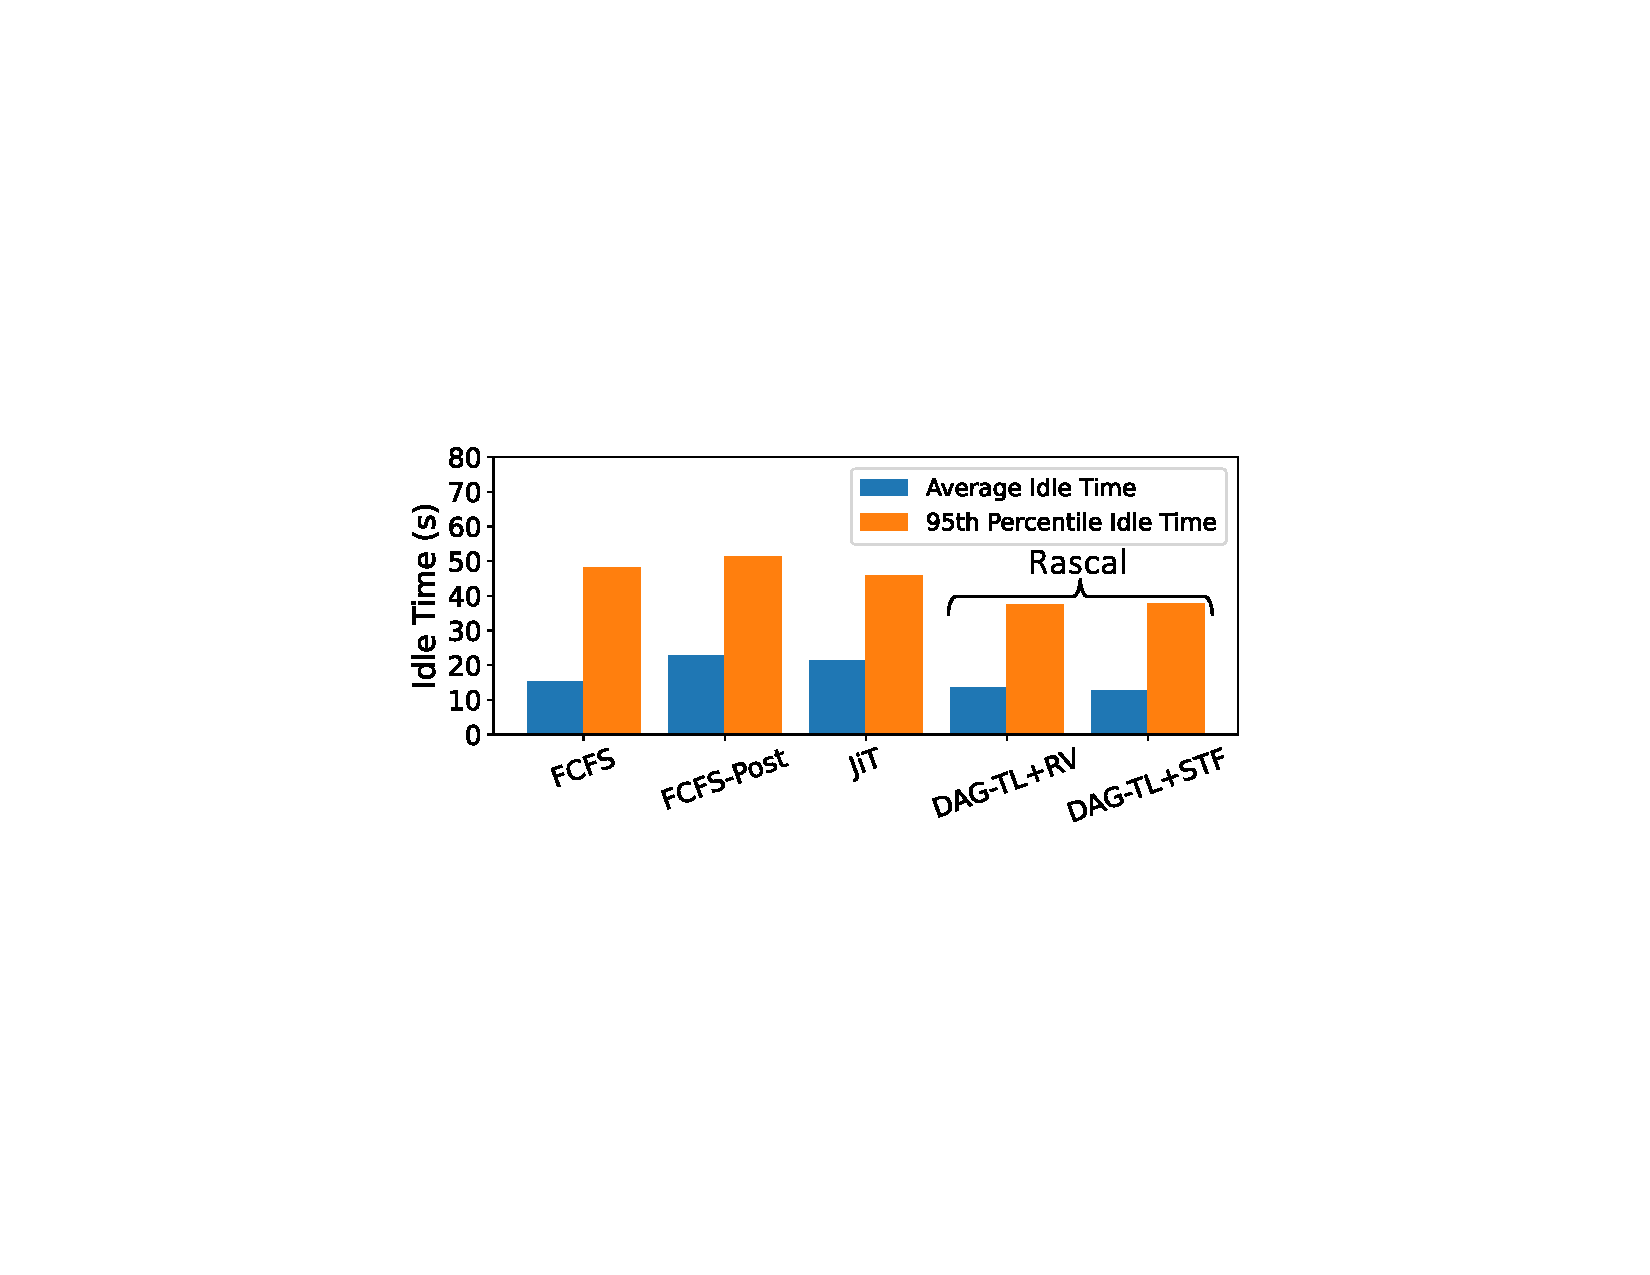
\includegraphics[width=\linewidth]{RASC/figures/evaluation/schedule_metric_Idle Time_rascal.pdf}
        \captionof{figure}{\small \bf Idle time comparison. \it \sysname{} achieves at least 27\% and 18\% lower mean and q95 values, resp.}
        \label{rasc:fig:idle_time_comparison}
    \end{minipage}
\end{figure}

\begin{figure}[t]
    \centering
    \begin{minipage}[t]{0.6\textwidth}
        \centering
        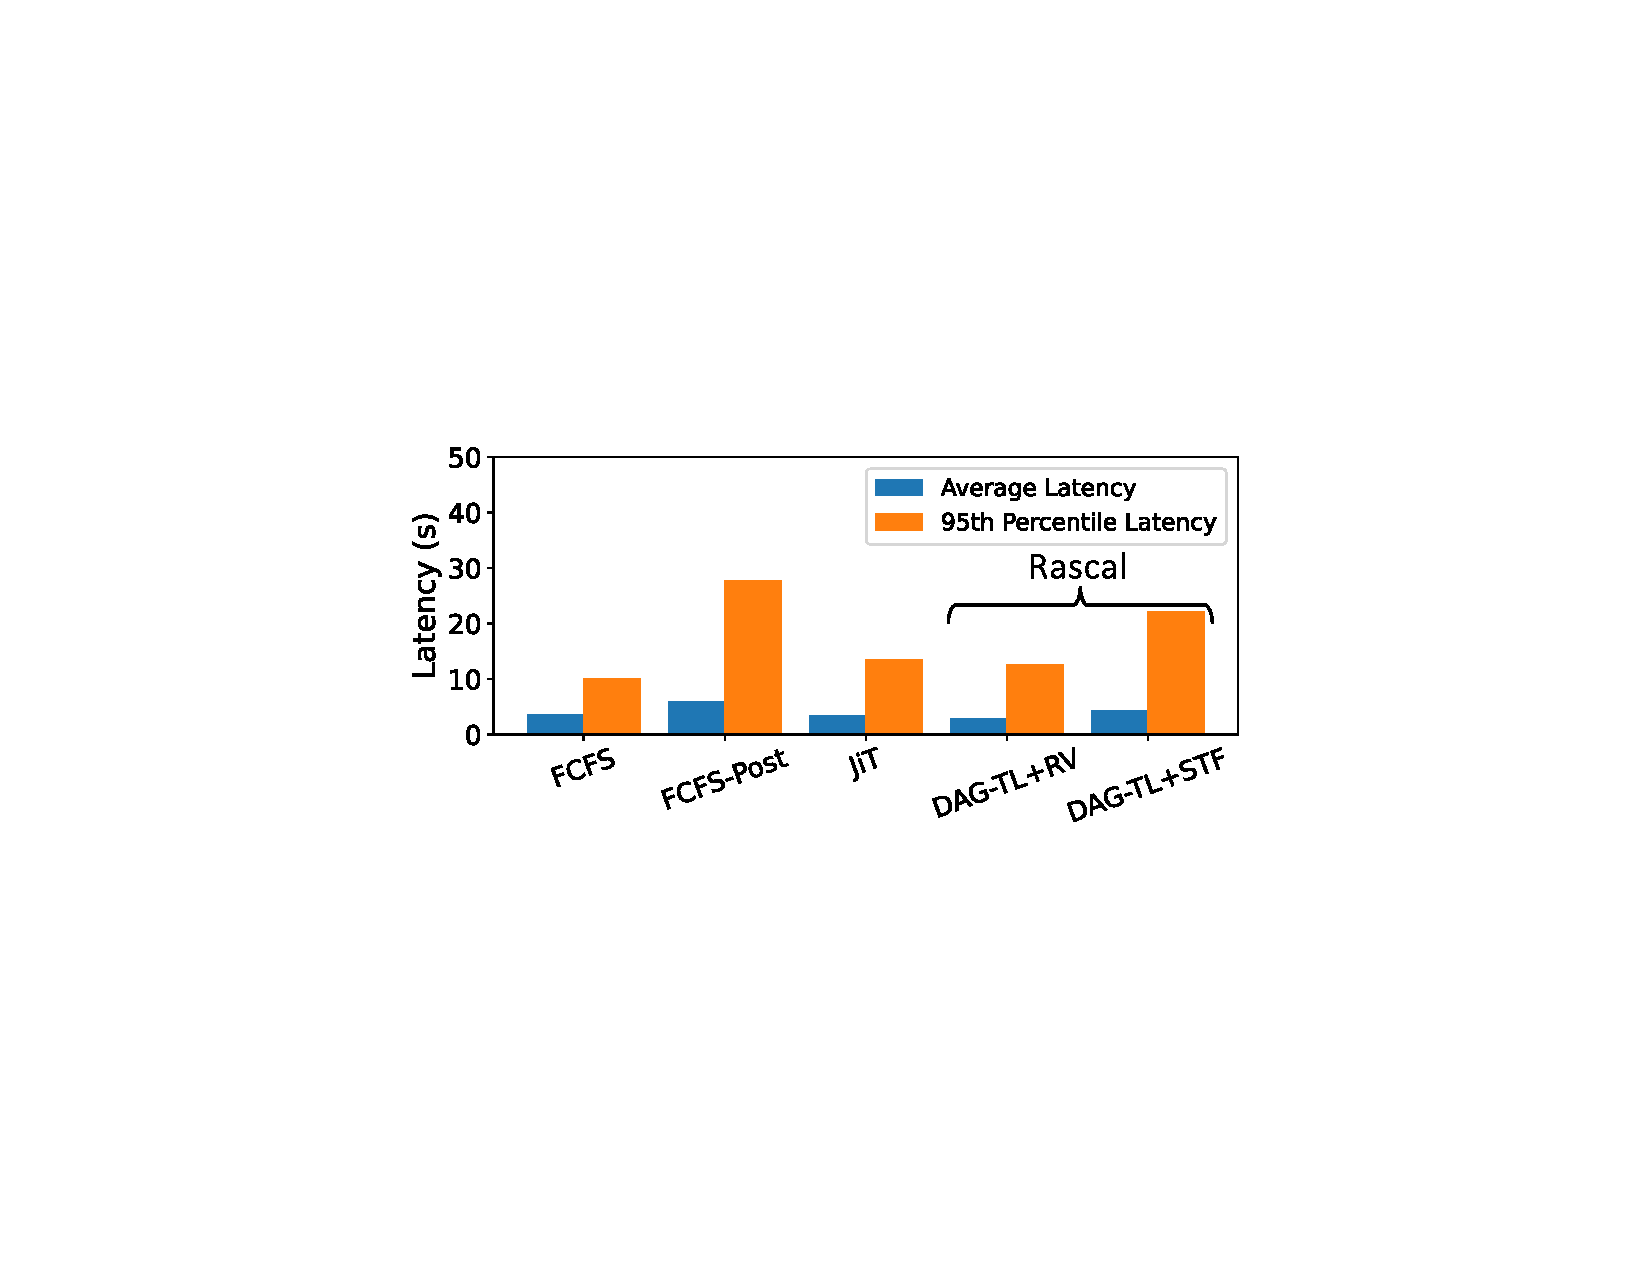
\includegraphics[width=0.87\linewidth]{RASC/figures/evaluation/schedule_metric_Latency_rascal.pdf}
        \captionof{figure}{\small \bf Latency comparison. \it \sysname{} achieves at least 25\% and 55\% lower mean and q95 values, resp.}
        \label{rasc:fig:latency_comparison}
    \end{minipage}
    \hspace{1cm}
    \begin{minipage}[t]{0.29\textwidth}
        \centering
        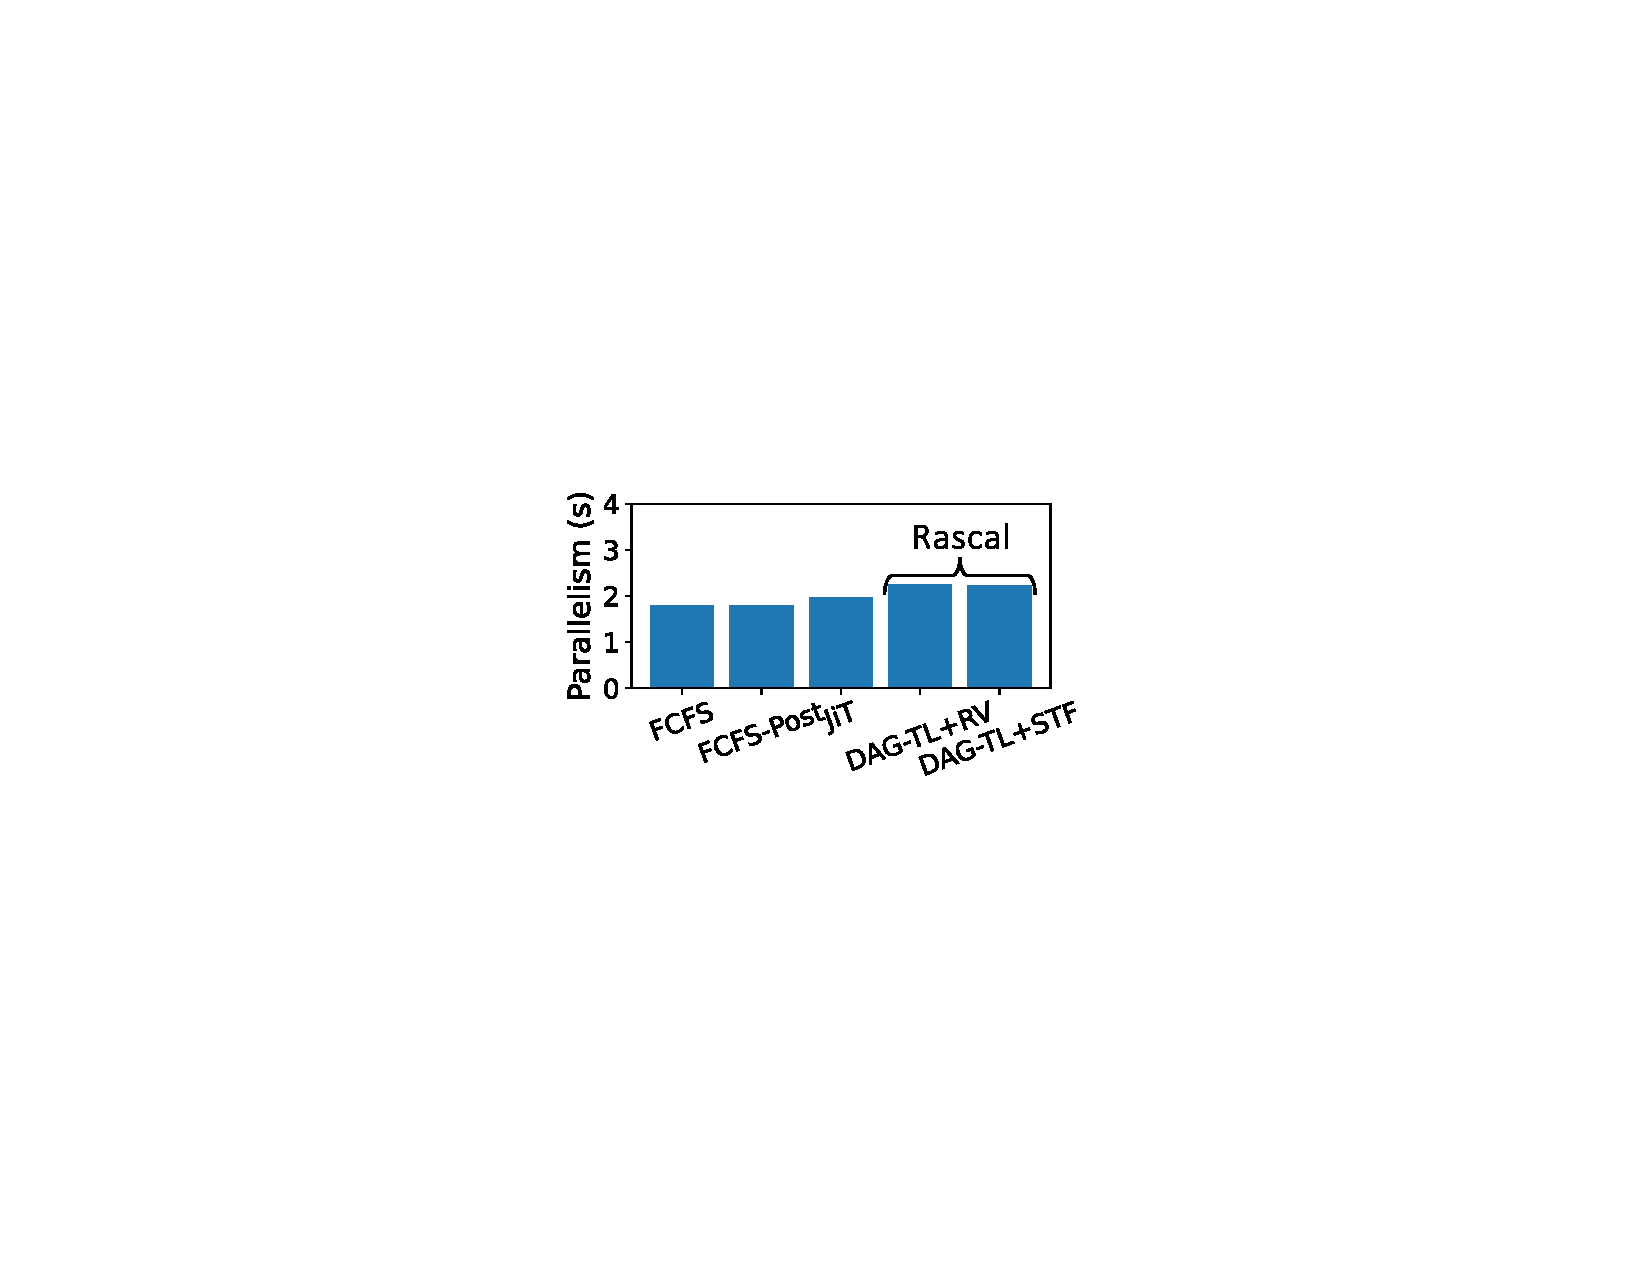
\includegraphics[width=\linewidth]{RASC/figures/evaluation/schedule_metric_Parallelism_rascal.pdf}
        \captionof{figure}{\small \bf Parallelism comparison. \it \sysname{} achieves $>$ 10\% parallelism.}
        \label{rasc:fig:parallelism_comparison}
    \end{minipage}
    % \caption{\bf \small Routine Benchmark on \sysname{} (right two bars in each plot) vs. Baselines (left three bars).} 
    % \label{rasc:routineresults1}
\end{figure}

\noindent \textbf{\sysname{} Rescheduler Vs. Baselines.} We compare two
\sysname{} reschedulers (STF and RV, \Cref{rasc:sec:rescheduler}: labeled in our plots as \scheduler+STF and \scheduler+RV respectively) against three baselines. 
Our three baselines are: (i)  FCFS (First Come First Served): 
strict no-overlap scheduling by arrival;
(ii) FCFS-Post: a faster FCFS variant allowing a routine to start 
once predecessor routines finish on all shared devices;
(iii) Just in Time (JiT) algorithm~\cite{SafeHomeEuroSys2021}, 
a greedy, opportunistic approach.


\Cref{rasc:fig:sched_len_comparison,rasc:fig:wait_time_comparison} show that 
(i) \sysname's two variants (\scheduler+RV and \scheduler+STF) perform similarly,
(ii) \sysname's slowest variant (\scheduler+STF) finishes routines 11\% faster than the fastest baseline (JiT), and
(iii) \sysname's slowest variant's wait times are also lower---mean by 33\% and q95 by 50\%---than the strongest baselines (JiT and FCFS, respectively).
\Cref{rasc:fig:idle_time_comparison} shows that \sysname{} reduces idle time (time a device is not utilized) by 27\% at mean and 18\% at 95th percentile compared to the fastest baseline (FCFS and JiT, respectively).
In \Cref{rasc:fig:latency_comparison}, \sysname{}'s slowest variant increases the routine end-to-end latency average time by only 25\% and 95th percentile by 55\%, compared to the fastest baseline (JiT and FCFS, respectively).
Finally, \Cref{rasc:fig:parallelism_comparison} shows that \sysname{}'s least efficient variant achieves 10\% higher average parallelism rates over the most efficient baseline (JiT). 
Overall, \sysname's rescheduling improves metrics by 10--55\% over baselines.
